\documentclass{article}
\usepackage{stmaryrd}
\usepackage{graphicx}

\title{Report, Kinetic project}
\author{Dorian Geraldes Pereira, Axel Demuth}
\date{March 2024}

\begin{document}
\maketitle
\tableofcontents
\newpage
\section*{Project Objective}

Within this project scope, the primary goal is to implement an efficient and accurate 
conversion process for Industry Foundation Classes (IFC) 
files representing buildings or cities into meshes compatible with the 
Kinetic algorithm. Subsequently, the Kinetic algorithm will be applied to these 
meshes to produce watertight models, facilitating the execution of finite element calculations.

The specific steps to be undertaken are as follows:

\begin{enumerate}   
    \item \textbf{Mesh Conversion:} From the IFC files we will have a 
    conversion in the stl or msh format,we will need to convert the STL 
    or MSH meshes into one of the formats accepted by the Kinetic algorithm, 
    such as .ply, .xyz, .las, .off.
    
    \item \textbf{Application of the Kinetic Algorithm:} Applicate  
    the Kinetic algorithm on the the converted 
    meshes to produce meshes optimized for finite element calculations.
    
    \item \textbf{Recovery of Material Labels:} Ensure the preservation 
    of information regarding materials present in the initial IFC-format mesh 
    and correctly associate them with elements of the converted mesh.
    
    \item \textbf{Utilization on City Modeling:} Extend the application of 
    the Kinetic algorithm to entire city models.
\end{enumerate}

\section*{Current Project Challenges}

Currently, the project faces several technical challenges:

\begin{enumerate}
    \item \textbf{Mesh Conversion:} Find a solutions to convert meshes 
    from STL or MSH files into one of the formats accepted by the Kinetic algorithm.
    
    \item \textbf{Parameter Optimization:} Identify and adjust appropriate 
    parameters to avoid segmentation faults and achieve satisfactory results 
    when applying the Kinetic algorithm.
    
    \item \textbf{Version Differences:} Understand the distinctions between 
    versions of the Kinetic algorithm,developed by CGAL and INRIA, to select 
    the right parameters to get the best result
\end{enumerate}

By overcoming these challenges, the project aims to provide a 
comprehensive and efficient solution for analyzing urban structures 
using the Kinetic algorithm to facilitate finite element calculations.\newline

\section{Tools}
\subsection{CGAL}
CGAL is a comprehensive package for geometry algorithms, providing various data structures and algorithms for working on polygons, surfaces, mesh generation, and more.
It offers a wide range of functionalities for geometric processing and analysis in various fields such as computer graphics, computational geometry, and geometric modeling.
\subsection{Kinetic}

Kinetic algorithms is a package from CGAL that allows working on meshes with some holes in them. When applied to the mesh, the Kinetic algorithms will 'extend' some surfaces to fill the mesh and make it watertight. 
Here's what the algorithm is capable of:


\begin{figure}[h]
    
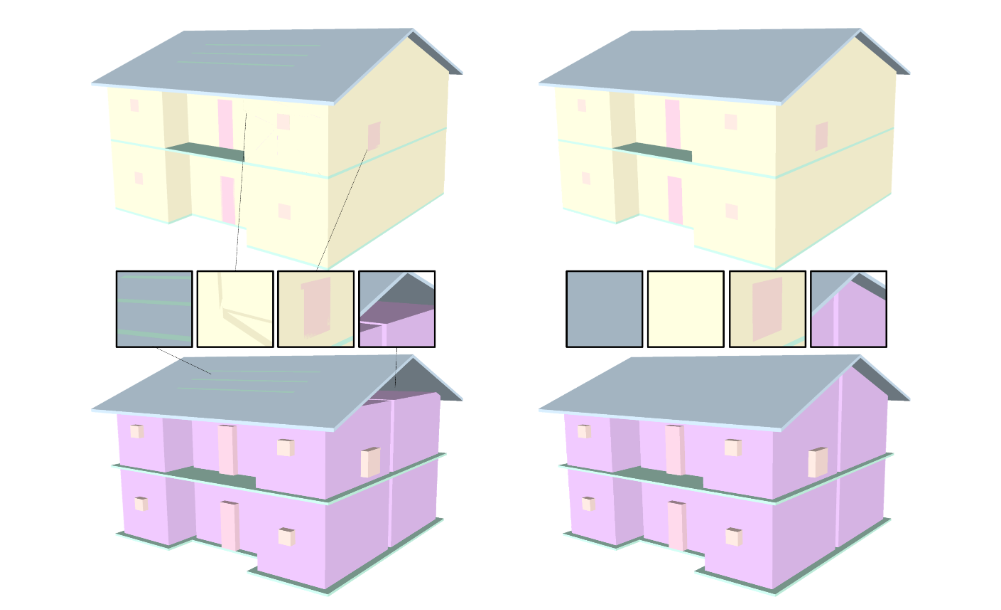
\includegraphics[scale =   0.3 ]{../images/example_algorithm.png}

\end{figure}



\subsection{Roadmap}
We intend to work on this project in the coming months and will continuously update our progress as outlined in the following roadmap.
\begin{figure}[h]
    
    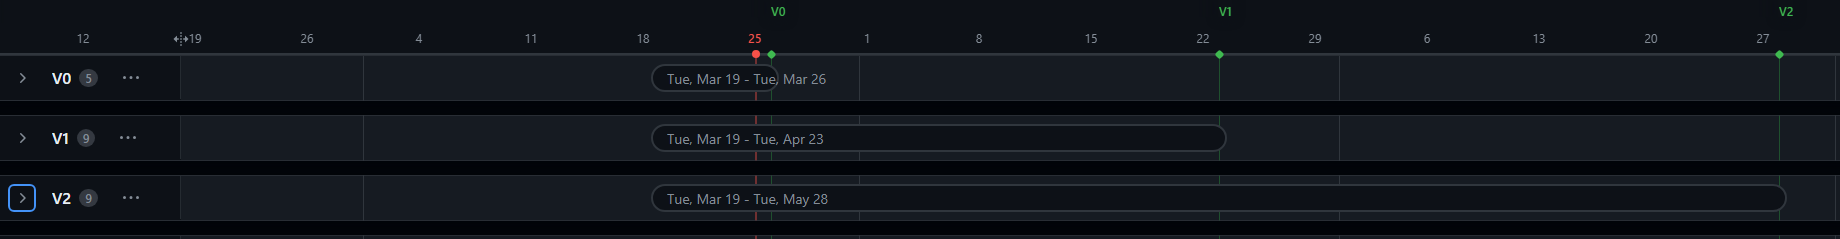
\includegraphics[scale =   0.3 ]{../images/roadmap.png}
    \end{figure}
    
\nocite{*}
\bibliographystyle{plain}
\bibliography{../bibliography/v0/report_bib}
\end{document}